\begin{appendices}
  \section{VPA Resource usage}
\begin{figure}[p]
  \centering
  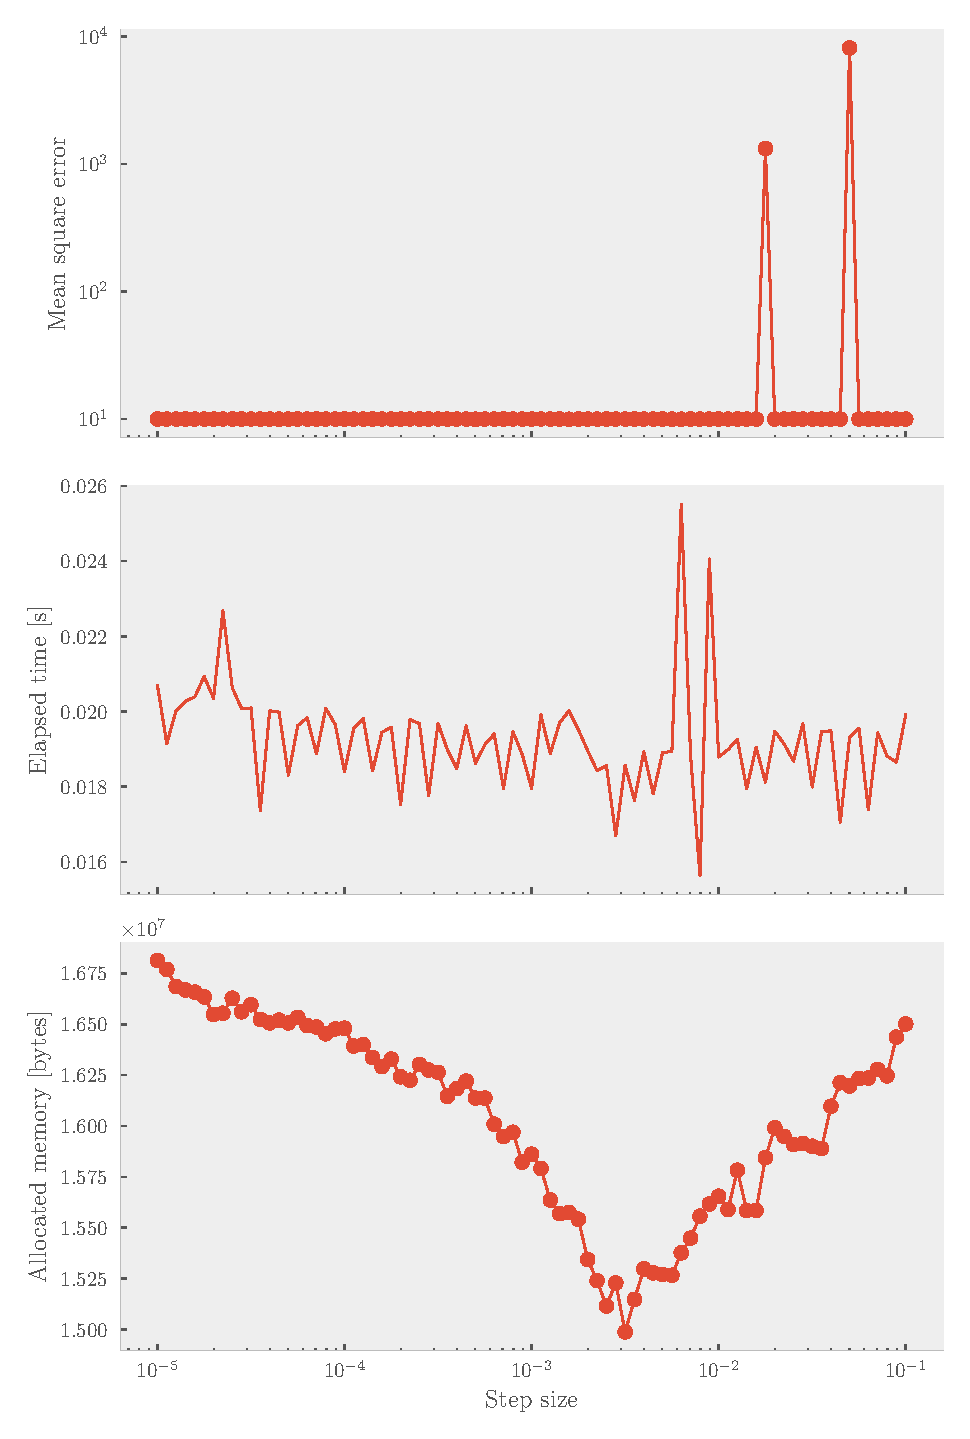
\includegraphics[]{Figures/vpa_measurements.pdf}
  \caption{\label{fig:vpa_measurements} Mean square error and resource usage of
    VPA as a function of step size of the solver. Only allocated memory has a
    significant change, reaching a minimum at \(0.008\)}
\end{figure}

\section{MSE curve for mass}
\begin{figure}[ht]
  \centering
  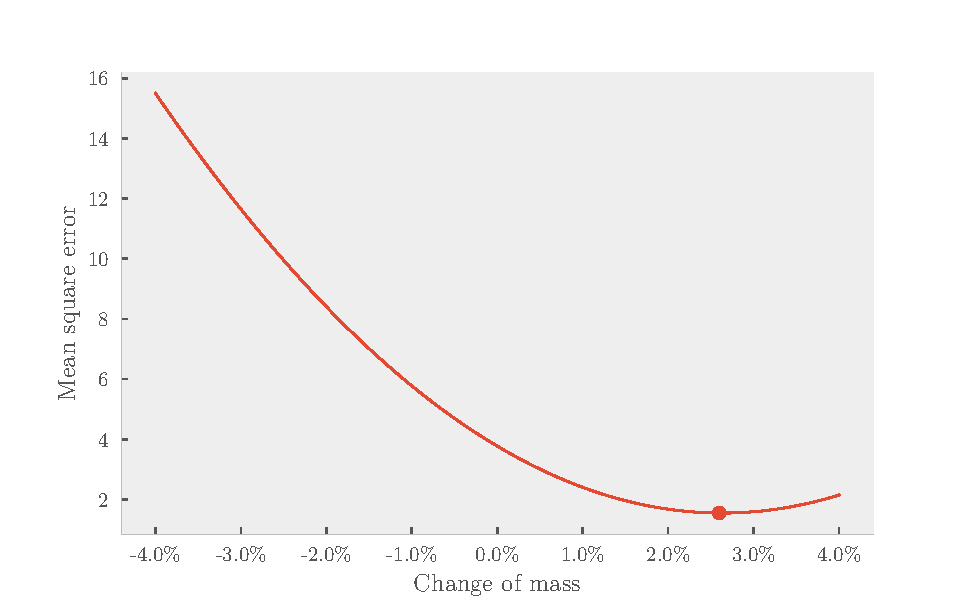
\includegraphics[]{Figures/optimal_mse.pdf}
  \caption{\label{fig:optimal_mse} The total MSE of each model using different
    mass. The minimum occurs at an additional \(+2.6\)\% mass, \SI{481.9}{MeV/c^2}.}
\end{figure}


\end{appendices}